%!TEX root = ../main.tex
\section{MPI-IO Hints Extensions}
\label{sec: e10-extensions}

To the best of our knowledge, at the time of writing this paper, there is very little or no work on how to use non-volatile memory devices in computing nodes of an HPC cluster as persistent cache layer to boost collective I/O performance in ROMIO. The use of these devices can greatly increase parallelism, reduce write response time variations among processes and consequently global synchronisation cost. Data cached in locally attached SSDs can be synchronised independently by every aggregator in the background while the application can progress doing useful work, effectively converting collective I/O to independent I/O when writing to the parallel file system.

To take advantage of attached non-volatile memories in computing nodes we introduced a new set of MPI-IO hints, reported in Table~\ref{table: hints_table}, and a corresponding set of modifications in the ROMIO implementation of the Universal File System (UFS) ADIO driver supporting them.

\begin{table}[!htb]
\centering
\ra{1.5}
\caption{Proposed MPI-IO hints extensions.}
\newcolumntype{K}{>{\centering\arraybackslash} m{4cm}}
\newcolumntype{V}{>{\centering\arraybackslash} m{4cm}}
\begin{tabular}{KV}
%\begin{tabular}{@{}p{0.55\columnwidth}p{0.43\columnwidth}@{}}
\toprule
\bf \small Hint & \bf \small Value \\
%\multicolumn{1}{c}{\bf \small Hint} & \multicolumn{1}{c}{\bf \small Value} \\
\midrule
\small \codeword{e10\_cache} & \small \codeword{enable}, \codeword{disable}, \codeword{coherent}\\
\small \codeword{e10\_cache\_path} & \small cache directory pathname\\
\small \codeword{e10\_cache\_flush\_flag} & \small \codeword{flush\_immediate}, \codeword{flush\_onclose}\\
\small \codeword{e10\_cache\_discard\_flag} & \small \codeword{enable}, \codeword{disable}\\
\small \codeword{ind\_wr\_buffer\_size} & \small synchronisation buffer size [bytes]\\
%\multicolumn{1}{c}{\small \codeword{ind\_wr\_buffer\_size}} & \multicolumn{1}{p{0.43\columnwidth}}{\centering \small synchronisation buffer size}\\
\hline
\end{tabular}
\label{table: hints_table}
\end{table}

The new hints are used to control the data path in the storage system as well as to define a basic set of cache policies for synchronisation and space management. In particular, the \codeword{e10\_cache} hint is used to \codeword{enable} or \codeword{disable} the cache, directing applications' data to the local file system instead of the global file system. When the hint is set to \codeword{coherent} all the written data extents will be locked until cache synchronisation is completed. The \codeword{e10\_cache\_path} hint is used to control where in the local file system tree the cache file will reside. The \codeword{e10\_cache\_flush\_flag} hint is used to control the synchronisation policy of cached data to the global file. If the hint is set to \codeword{flush\_immediate} data will be immediately flushed to the global file. Alternatively, if the hint is set to \codeword{flush\_onclose} data will be flushed to the global file when it is closed. The \codeword{e10\_cache\_discard\_flag} hint is used to perform basic cache space management. In particular, if the hint is set to \codeword{enable} the cache file will be removed after the file is closed, otherwise (\codeword{disable}) it will be retained until the user manually removes it. Finally, the \codeword{ind\_wr\_buffer\_size} hint controls the size of the buffer used to synchronise cached data to the global file. This hint already existed in ROMIO but was only used during independent I/O to determine the write granularity. The hints in Table~\ref{table: hints_table} can be used in conjunction with the collective I/O hints described in Section~\ref{subsec: hints}.

Besides the proposed cache policies, more complex ones are possible. For example, the cache synchronisation could take into account the level of congestion of the I/O servers. The cache replacement policy could also use a more complex strategy to evict cached files (or extents of data inside the file). Although these can be implemented in ROMIO, they introduce more sophisticated functionalities that go beyond the scope of this work.

\subsection{Cache Hints Integration in ROMIO}
\label{subsec: support}
As already mentioned, the introduced MPI-IO hints are supported by a corresponding set of modifications in the ROMIO implementation~\cite{E10-DEEPER}. These modifications, following described, provide the functionalities necessary to handle the additional cache layer:

\begin{itemize}
        \item \codeword{ADIOI\_Sync\_thread\_start()}: is a new implemented routine providing cache synchronisation in ROMIO. It uses a dedicated POSIX thread to read data back from the cache file into the synchronisation buffer, and write it to the global file;
        \item \codeword{ADIOI\_Cache\_alloc()}: is a new implemented routine providing cache space allocation in ROMIO. It uses the \codeword{fallocate()} system call to efficiently allocate space in the local file system\footnote{For file systems that do not support the fallocate syscall the implementation reverts to standard allocation methods which physically writes zeros to the file, at the cost of time efficiency.};
        \item \codeword{ADIOI\_GEN\_OpenColl()}: is the routine providing collective file open in ROMIO. In the new implementation, when \codeword{e10\_cache} is set to \codeword{enable}, this routine also opens the cache file and stores its MPI file handle in the \codeword{cache\_fd} field, added for the purpose inside the global MPI file handle. If for any reason the open of the cache file fails, the implementation reverts to standard open;
        \item \codeword{ADIOI\_GEN\_WriteContig()}: is the routine providing contiguous file write in ROMIO. In the new implementation, when \codeword{e10\_cache} is set to \codeword{enable}, this routine uses the \codeword{cache\_fd} file handle to write data. Additionally, it creates a synchronisation request (with associated \codeword{MPI\_Request} handle) for the written extent~\cite{mpispecs} and sends it to \codeword{ADIOI\_Sync\_thread\_start()}, which will take care of moving data to the global file system. When data transfer is complete the sync function invokes \codeword{MPI\_Grequest\_complete()} on the \codeword{MPI\_Request} handle associated with the request;
        \item \codeword{ADIO\_Close()}: is the routine providing file close in ROMIO. In the new implementation, when \codeword{e10\_cache} is set to \codeword{enable}, this routine also invokes the \codeword{ADIOI\_GEN\_Flush()} routine to make sure that all the data in the cache has been moved to the global file system, and finally closes the cache file as well as the global file;
        \item \codeword{ADIOI\_GEN\_Flush()}: is the routine providing file flushing in ROMIO. In the new implementation, when \codeword{e10\_cache\_flush\_flag} is set to \codeword{flush\_immediate}, it takes care of checking that previously created synchronisation requests have been completed by invoking \codeword{MPI\_Wait()} on the associated \codeword{MPI\_Request} handle. Alternatively, when \codeword{e10\_cache\_flush\_flag} is set to \codeword{flush\_onclose}, it sends all the pending synchronisation requests to \codeword{ADIOI\_Sync\_thread\_start()} and then waits for them to complete as described above.
\end{itemize}

%In particular, the \codeword{ADIOI\_GEN\_OpenLocal} routine opens the file in the local file system cache to which data will be written. The local pathname is computed as the base name of the global pathname, prefixed with the pathname passed by the user through the \codeword{e10\_cache\_path} hint. Thus, if the file has global \codeword{pathname} = \codeword{/user1/project1/foo} and \codeword{e10\_cache\_path} = \codeword{/tmp/user1/project1}, the local pathname will be \codeword{/tmp/user1/project1/foo}. Of course, local opens can possibly fail for a number of reasons (e.g. the local pathname passed by the user does not exist). In all these cases the implementation will revert to standard collective I/O resetting the \codeword{e10\_cache} hint to \codeword{disable}.
%If the file in the local file system is opened successfully, data is written to it using the \codeword{ADIOI\_GEN\_WriteContigLocal} routine which replaces \codeword{ADIOI\_GEN\_WriteContig} in the diagram in Figure~\ref{figure: coll_io_impl}.

%The \codeword{ADIOI\_GEN\_IfileSync} routine is responsible for the synchronisation of the local cache file to the global file system. Depending on the value of the flush hint it will be invoked immediately after \codeword{MPI\_File\_write\_all} returns from writing all the data to the local cache (\codeword{flush\_immediate}), see Figure~\ref{figure: coll_io}, or at close time (\codeword{flush\_onclose}). The difference is that in the first case the application can progress with computation while the non-blocking synchronisation routine does its job. In the second case, on the other hand, the implementation will busy wait until synchronisation is complete before returning the control to the application. The \codeword{ADIOI\_GEN\_IfileSync} routine is implemented using the MPI Generalised Request interface~\cite{mpispecs}, which allows users to write non-blocking routines as well as call back functions to be used by the MPI implementation to control the state and the progress of an additional user thread through the \codeword{MPI\_Request} object and \codeword{MPI\_Wait} function. 
%In our implementation we use a pthread to synchronise the content of the local file with the parallel file system.%The \codeword{ind\_wr\_buffer\_size} hint, previously mentioned, is used by the synchronisation routine to set the size of the buffer used to read data from the local file and write it to global file, and thus affects the number of synchronisation rounds.

%The \codeword{ADIOI\_GEN\_CloseLocal} routine is used to close the local cache file and start data synchronisation if \codeword{e10\_cache\_flush\_flag} = \codeword{flush\_onclose}. Finally, the \codeword{ADIO\_CacheAlloc} routine is used by aggregators to reserve space in the local cache file system. The routine uses the \codeword{fallocate} system call to allocate space in the file system's data structures instead of writing data to the file, and is therefore more time efficient\footnote{For file systems that do not support the fallocate syscall the implementation reverts to standard allocation methods which physically writes zeros to the file, at the cost of time efficiency.}. If there is not enough space available in the cache, the implementation will revert to standard collective I/O, resetting the \codeword{e10\_cache} to \codeword{disable}.

\subsection{Consistency Semantics}
\label{subsec: consistency}
As far as write consistency is concerned, the MPI-IO interface does not make any assumption regarding the underlying storage system or its semantics. ROMIO specifically supports file systems that are both POSIX compliant, like Lustre, and non-POSIX compliant, like NFS or PVFS. In MPI-IO, written data becomes globally visible only after either \codeword{MPI\_File\_sync()} or \codeword{MPI\_File\_close()} are invoked on the MPI file handle and by default there is no write atomicity. The motivation is that data can be cached at some level locally in the compute nodes. The ROMIO implementation can overcome the risk of data inconsistency, e.g. related to false sharing of file system blocks, using persistent file realms~\cite{ColomaCWWRP04}, and can even enforce atomicity using \codeword{MPI\_File\_set\_atomicity()}.

In our implementation we comply to the MPI-IO semantics just described. This means that data written to the local file system cache using the newly introduced MPI-IO hints will be globally visible to the rest of the nodes only under the following circumstances:
\begin{itemize}
\item The \codeword{e10\_cache\_flush\_flag} has been set to \codeword{flush\_immediate} by the user and synchronisation, started automatically by the implementation right after the write operation, has completed;
\item The \codeword{e10\_cache\_flush\_flag} has been set to \codeword{flush\_onclose} by the user and the invoked \codeword{MPI\_File\_close()} has returned;
\item The \codeword{MPI\_File\_sync()} function has been invoked by the user and it has returned.
\end{itemize}

%At any time users can make sure their data is persistent by invoking \codeword{MPI\_File\_sync} on the MPI file handle. This will call the \codeword{ADIOI\_GEN\_FlushLocal} routine, previously described, that returns only after all the cached data has been synchronised to the global file system or immediately if synchronisation has been already completed. This is perfectly aligned with the MPI-IO consistency semantic which also requires the invocation of \codeword{MPI\_File\_sync} or \codeword{MPI\_File\_close} to ensure that local cached data is persistent in the global file system.

Consistency for reading data from the cache is not clearly defined by the ext2ph algorithm. In general, data written to the local file system cache can be read back from the user without accessing the global file system. Nevertheless, the algorithm calculates the location of a data block based on the number of aggregators, their logical position within the set of aggregators, and the size of the complete data set. This means that a collective read that matches the previous write could safely read the data from the aggregators' cache without incurring any problem. In spite of that, in general reading from the cache requires additional metadata describing the file layout across the caches. For this reason, we currently do not support reads from the local file system cache.

%In general, data written to the local file system cache could be read back from the user without accessing the global file system. Nevertheless, the local cache file in each aggregator only contains the corresponding file domain, which can vary with the number of processes used to run the experiment as well as the number of aggregators selected. This means that a collective read that matches the configuration (number of aggregators) and I/O pattern of the previous write could safely read the data from the aggregators' cache without incurring into any problem. In spite of that, in general reading from the cache requires additional metadata describing the file layout across the caches. For this reason, we currently do not support reads from the local file system cache. %Instead, it is responsibility of the user to make sure that data is persistent in the global file system before reading it back (i.e. by closing the file or flushing the cache content).
%Most HPC applications are simulation codes that have write dominated I/O patterns. They write data to a shared file (or multiple files) for later post processing or defensive checkpoint restart and then progress with computation. Data is typically not read back during normal execution and thus cache coherency is not required. In any case, 

Furthermore, whenever required, we can enforce cache coherency ensuring that read operations cannot access data that is currently in transit, i.e., not or only partially moved from the cache to the global file. This can be done by locking the file domain extent being cached until all the data has been made persistent in the global file. For this purpose ROMIO provides a set of internal locking macros, namely \codeword{ADIOI\_WRITE\_LOCK}, \codeword{ADIOI\_READ\_LOCK} and \codeword{ADIOI\_UNLOCK} that we used in our implementation. The lock of cached data can be selected by setting the \codeword{e10\_cache} hint in Table~\ref{table: hints_table} to \codeword{coherent}. This will \codeword{enable} the cache and set locks appropriately, assuming underlying file system support.

%Typically, if ROMIO can detect stripe size and stripe factor for the file, it will automatically align file domains to the file system stripe, avoiding concurrent locking of the same block by multiple aggregators. In this case, the enforcement of cache coherency through locking will not degrade performance.
%Currently, in order to avoid partially synchronised files, i.e. in the case of a node failing, for new files, the global pathname is hidden at the time of open and made visible again only after close, once all the data has been synchronised and consistency is ensured. If the file already exists, on the other hand, its pathname is not altered. 

\subsection{Changes to the Application's Workflow}
\label{subsec: new-workflow}
Simplifying, most HPC applications can be divided into multiple phases of computation, in which data is produced, and I/O, in which data is written to persistent storage for post-processing purposes as well as defensive checkpoint-restart. Focusing on the I/O phase and considering the case of applications writing to a shared file, the I/O phase can be divided into the following steps:
\begin{enumerate}
        \item The file is opened using \codeword{MPI\_File\_open()}: at this point the info object containing the user defined MPI-IO hints is passed to the underlying ROMIO layers.
        \item Data is written to the file using \codeword{MPI\_File\_write\_all()}: these functions invoke the underlying \codeword{ADIOI\_GEN\_WriteStridedColl()} previously described in Figure~\ref{figure: coll_io_impl}.
        \item The file is closed using \codeword{MPI\_File\_close()}: after the file is closed data must be visible to every process in the cluster. 
\end{enumerate}

To take advantage of the proposed MPI-IO hint extensions, the application's workflow has to be modified. Figure~\ref{figure: workflow3} shows the classical application's workflow (cache disabled) as well as the modified version using the new hints (cache enabled). The difference is that, in order to take advantage of the proposed hints and hide the cache synchronisation to the computation phase, the \codeword{MPI\_File\_close()} for the I/O phase `k' has been moved at the beginning of the I/O phase `k+1', just before the new file is opened.
\begin{figure}[!htb]
  \centering
  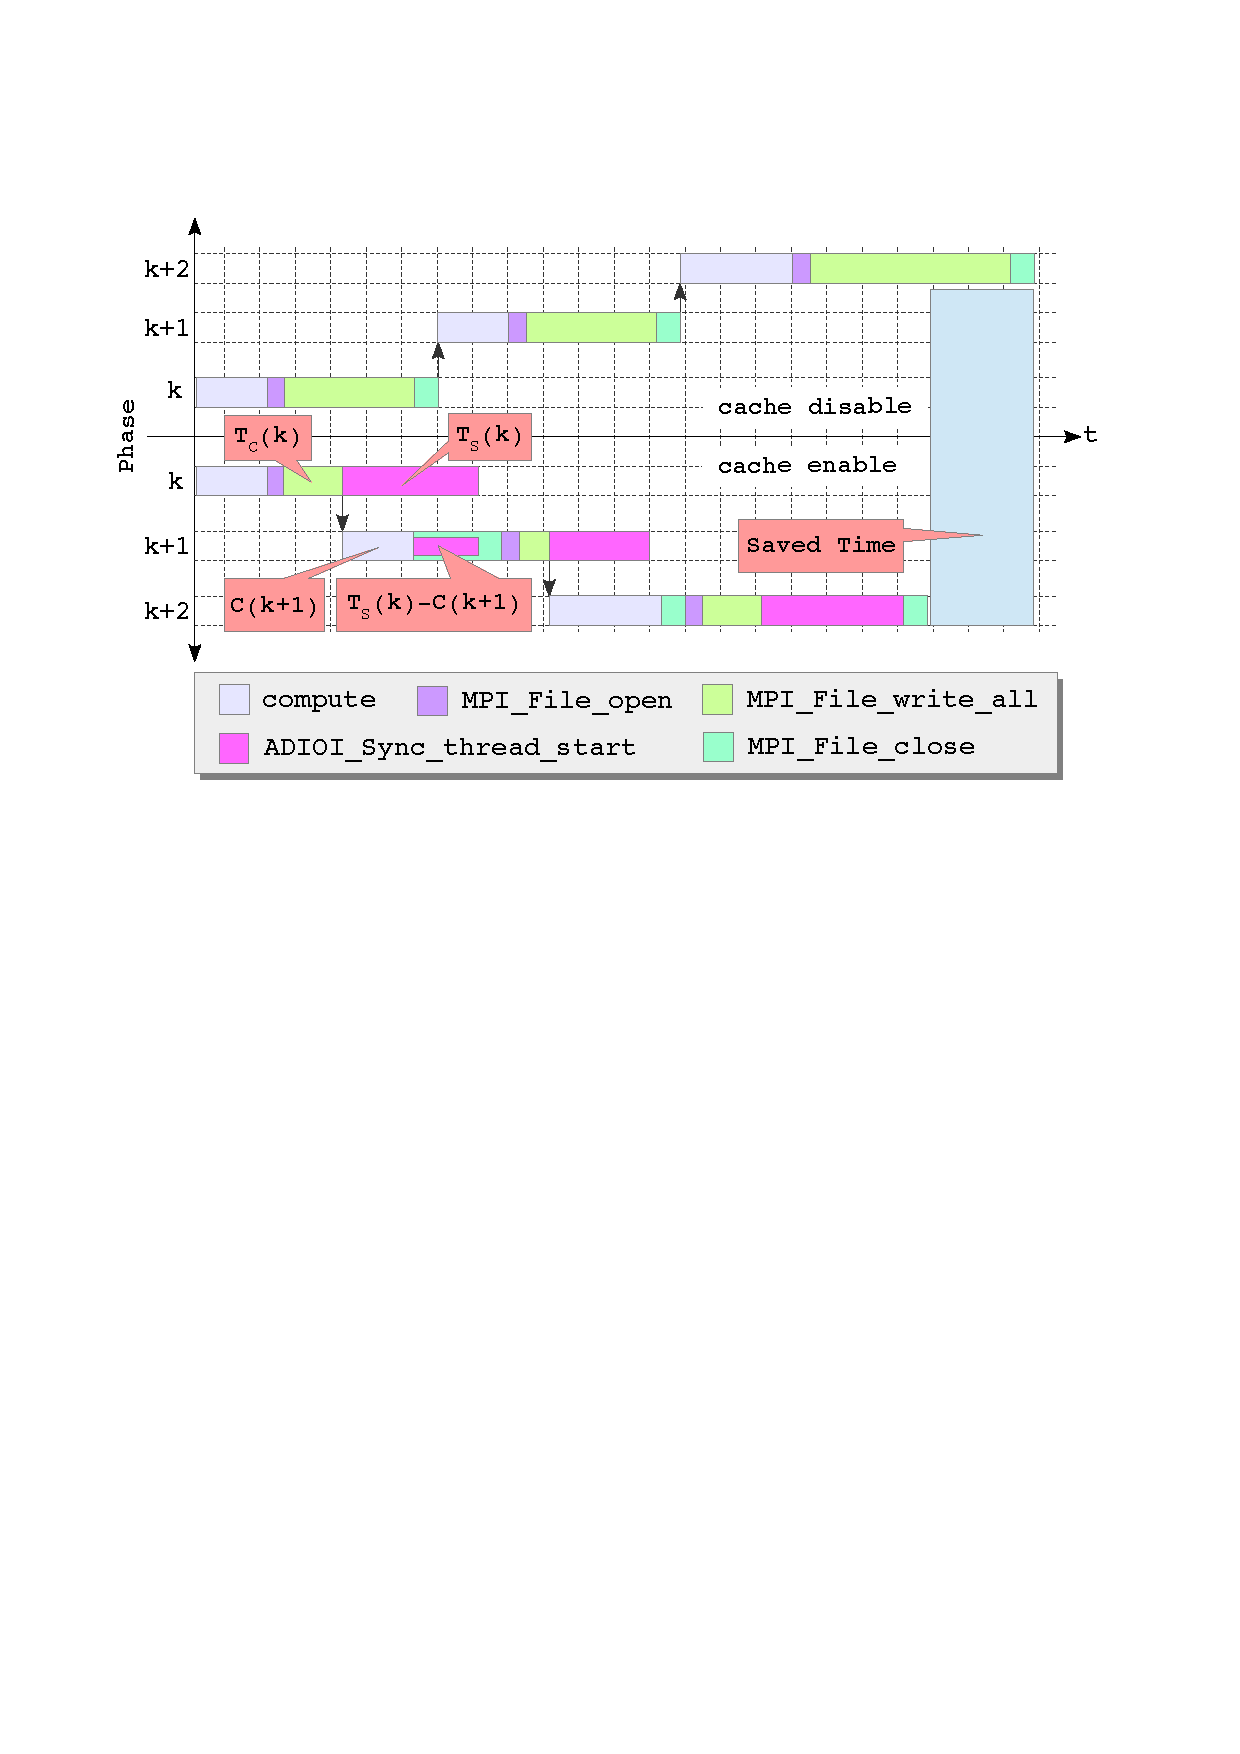
\includegraphics[width=\columnwidth]{figures/workflow3}
  \caption{Standard and modified workflows. When cache is disabled compute phase `k+1' starts after file `k' has been closed. When the cache is enabled compute `k+1' can start immediately after data has been written. At the same time, background synchronisation of cached data starts. File `k' is closed before the file `k+1' is opened, forcing the implementation to wait for cache synchronisation to complete.}
  \label{figure: workflow3}
\end{figure}

Since the workflow modification just presented might not be feasible for legacy applications, we developed a MPI-IO wrapper library (called MPIWRAP), written in C++, that can reproduce this change behind the scenes. The library can be linked to the application or preloaded with \codeword{LD\_PRELOAD} and has been used for all the experiments contained in this paper. MPI-IO hints are defined in a configuration file and passed by the library to \codeword{MPI\_File\_open()}. We can define multiple hints targeting different files or groups of files. The library overloads \codeword{MPI\_\{Init,Finalize\}()} and \codeword{MPI\_File\_\{open,close\}()} using the PMPI profiling interface. The workflow modification can be triggered for a specific set of files (identified by the same base name) in the configuration file. Whenever one of such files is closed, our \codeword{MPI\_File\_close()} implementation will return success. Nevertheless, the file will not be really closed. Instead, its handle will be kept internally for future references. When the next shared file with the same base name is opened, our \codeword{MPI\_File\_open()} implementation will search for outstanding opened file handles and will invoke \codeword{PMPI\_File\_close()} on them before opening the new file, thus triggering the cache synchronisation completion check for each of them.

\subsection{I/O Bandwidth}
\label{subsec: bw-impr}
According to the new I/O workflow, described in this section, we have that being $S(k)$ the amount of data written during phase `k', $T_c(k)$ the time needed to write $S(k)$ collectively to the cache using \codeword{MPI\_File\_write\_all()}, $T_s(k)$ the time needed to synchronise the cached data in every aggregator to the global file system (through \codeword{ADIOI\_Sync\_thread\_start()}), and $C(k+1)$ the computation time of phase `k+1', the resulting I/O bandwidth for `k' is expressed by Equation~\ref{formula: bw}:

\begin{equation}\label{formula: bw}
        bw(k) = \frac{S(k)}{T_c(k) + max(0,\ T_s(k) - C(k+1))} \\
\end{equation}
Therefore, the total average bandwidth perceived by the application is:
\begin{equation}\label{formula: abw}
        BW = \frac{\sum_{k=0}^{N-1} S(k)}{\sum_{k=0}^{N-1} T_c(k) + max(0,\ T_s(k) - C(k+1))}
\end{equation}

From Equation~\ref{formula: bw} (in which we have considered the open time neglectable) it is clear that the maximum performance can be obtained when $C(k+1) \geq T_s(k)$, that is, when we can completely hide cache synchronisation by the computation phase. On the other hand when $C(k+1) < T_s(k)$ we might have a minima in the bandwidth since \codeword{MPI\_File\_close()} needs to wait for cache synchronisation completion (Figure~\ref{figure: workflow3}). 
%Finally, being $T_g$ the standard collective write time to the global file system, we assume that $T_g >> T_c$. This assumption is legitimated by the fact that in very large scale systems the number of compute nodes (and thus the number of NVM devices) is orders of magnitude bigger than the available storage targets.
